\section{Introduction}

<<<<<<< HEAD
\indent This report presents the initial work developed in the project, between march and may. On the long term, the objective of this project is to be able to simulate the propagation of water waves using a numerical model, understood as an algorithm or computer program, that can capture the physics associated to all different scales and phenomena, from the ocean to the shore and also including the intrinsic variability in the generation process of water waves. The methodology that has been chosen for this goal is to couple different models that are currently known as the best representation for the physics associated to each scale, by means of developing proper boundary conditions. Hence the interest of the study is split in two parts that are being run in parallel: first to get some familiarity with the equations and the physics we want to represent, and second, to get introduced to the study of the boundary conditions that will serve as communicators between our models.

The work that has been done from March to May has focused mainly on the study and implementation of nonlinear dispersive models for wave propagation: the KdV, BBM and Serre equations. In sections \ref{sec:KdV} to \ref{sec:Serre}, we describe each one of these models, the theoretical study performed (for example, a scale analysis for the KdV equation) and the proposed discretizations for their computational resolution, using splitting schemes combining finite volume and spectral or finite difference methods. Some examples are presented to illustrate the numerical results and show the problems that must be corrected in the schemes.

\indent Then, in section \ref{sec:TBC} we move to the other topic of interest which is the study of Transparent Boundary Conditions (TBC's). There, we describe a first approach and then proceed with the study of simple approximations to the TBC's in the case of the KdV equation.

\subsection{Motivation example}

In this section we show the importance of boundary conditions when modeling water waves propagation for the particular case of tsunami waves, using the free open source software GeoClaw \cite{geoclaw} developed in the University of Washington, which uses a well-balanced shock capturing finite volume scheme with variable Adaptive Mesh Refinement (AMR) for the space discretization.

The simulation corresponds to the tsunami that struck the coast of Chile the year 2010 and two different domains have been chosen such that one is the extension of the other from the left boundary. Both domains, with their respective bathymetry and topography distribution, are shown in figure \ref{intro:topobati}, and each domain is defined in geographic latitude and longitude coordinates by $\Omega_1 = \{ (x,y)\in[-120,-60]\times[-60,0] \}$ and $\Omega_2 = [-170,-60]\times [-60,0]$. Neumann boundary conditions are used for both domains, and the idea is to compare the values on the left boundary of $\Omega_1$ with respect to those obtained there with $\Omega_2$.

\begin{figure}
	\center
	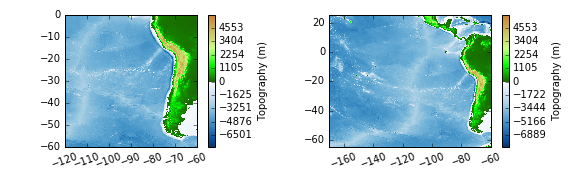
\includegraphics[width=\textwidth]{figures/GeoclawChile2010_domains_topo.png}
	\caption{Topography and Bathymetry for domains $\Omega_1$ and $\Omega_2$ used in the simulations}
	\label{intro:topobati}
\end{figure}

The initial conditions are defined as zero velocity and the deformation for the water free surface shown in figure \ref{intro:qinit} is the same as the seafloor deformation calculated by the dislocation model of Okada \cite{okada1985surface}, using the fault parameters listed in table \ref{intro:faulttable} proposed by the USGS for this case. The grid resolution is chosen as $\Delta x = \Delta y = 0.5$ degrees and the model is forced to not to use grid refinement. 

\begin{table}[]
\centering
\caption{My caption}
\label{my-label}
\begin{tabular}{|l|l|}
\hline
\textbf{Lat (degrees)}    & -72.668 \\ \hline
\textbf{Lon (degrees)}    & -35.826 \\ \hline
\textbf{Length (km)}      & 450     \\ \hline
\textbf{Width (km)}       & 100     \\ \hline
\textbf{Strike (degrees)} & 16      \\ \hline
\textbf{Depth (km)}       & 35      \\ \hline
\textbf{Slip (m)}         & 15      \\ \hline
\textbf{Rake (degrees)}   & 104     \\ \hline
\textbf{Dip (degrees)}    & 14      \\ \hline
\end{tabular}
\label{intro:faulttable}
\end{table}

\begin{figure}
	\center
	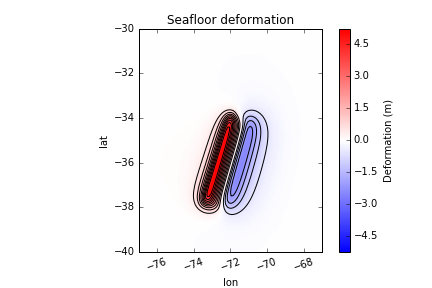
\includegraphics[width=0.5\textwidth]{figures/GeoclawChile2010_faultUinit.png}
	\caption{Deformation used for both the seafloor and free-surface of the water as initial condition.}
	\label{intro:qinit}
\end{figure}

Figures \ref{intro:results_frame23}, \ref{intro:results_frame28}, and \ref{intro:results_frame35} show the results of the simulations using $\Omega_1$ and $\Omega_2$ and the differences between $\Omega_1$ and $\Omega_2$ for the values of the free surface when the wave meets and leaves the boundary. From the values of the differences we can see that inside the domain there is some errors far from the boundaries that can be explained by both output interpolation of the software GeoClaw and the differences in fluxes at the boundaries of the patches that GeoClaw uses for managing the AMR, even when imposing fixed grids in the simulation. However it is possible to observe that the most important differences come from spurious reflection with the artificial boundary used in $\Omega_1$. These differences reached a magnitude of the order of $1cm$, which can be comparable, if not with that of the leading front, possibly with secondary waves that can remain after the first arrival.

Thus, here we have shown that with the simple approach of using Neumann boundary conditions to represent open or transparent boundary conditions, some differences can be observed with respect to using a bigger domain in the simulation, and then, some improvement can be done to decrease the magnitude of these differences.



\begin{figure}
	\center
	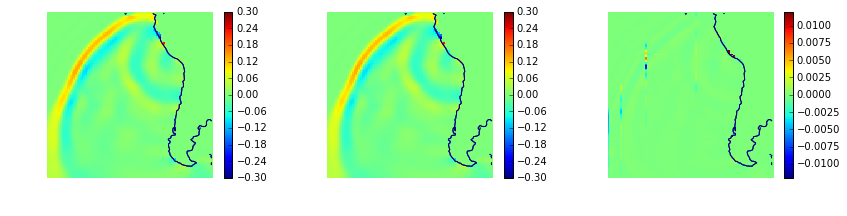
\includegraphics[width=\textwidth]{figures/GeoclawChile2010_comparison_it23}
	
	\caption{Comparison of the free surface elevation in the region $\Omega_1$, for simulations using the small domain $\Omega_1$ (left), big domain $\Omega_2$ (center), and the difference between both of them (right), at $t=5.75$ hours.}
	\label{intro:results_frame23}
\end{figure}

\begin{figure}
	\center
	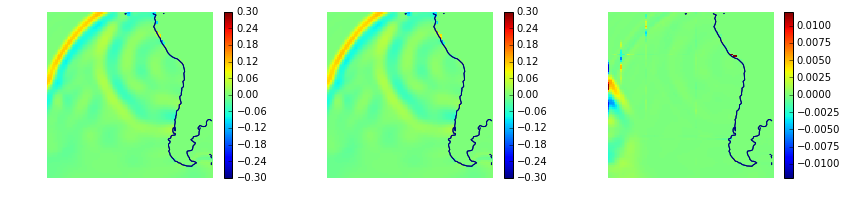
\includegraphics[width=\textwidth]{figures/GeoclawChile2010_comparison_it28}
	\caption{Comparison of  the free surface elevation in the region $\Omega_1$, for simulations using the small domain $\Omega_1$ (left), big domain $\Omega_2$ (center), and the difference between both of them (right), at $t=7.00$ hours.}
	\label{intro:results_frame28}
\end{figure}

\begin{figure}
	\center
	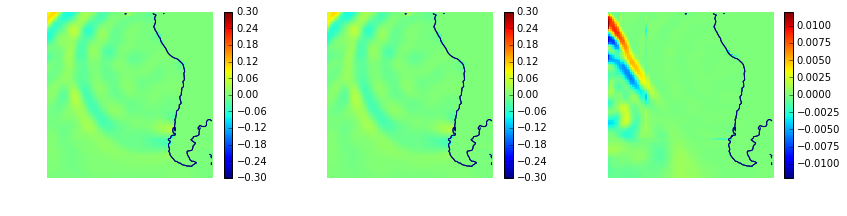
\includegraphics[width=\textwidth]{figures/GeoclawChile2010_comparison_it35}
	\caption{Comparison of the free surface elevation in the region $\Omega_1$, for simulations using the small domain $\Omega_1$ (left), big domain $\Omega_2$ (center), and the difference between both of them (right), at $t=8.75$ hours.}
	\label{intro:results_frame35}
\end{figure}
=======
\indent This report presents the initial work developed in the project, between March and May. It was mainly focused on the study and implementation of nonlinear dispersive models for wave propagation: the KdV, the BBM and the Serre equations. In the sections \ref{sec:KdV} to \ref{sec:Serre}, we describe each one of these models, the theoretical study realized (for example, a scale analysis for the KdV equation) and the proposed discretizations for their computational resolution, using splitting schemes combining finite volume and spectral or finite difference methods. Some examples are presented to illustrate the numerical results and show the problems that must be corrected in the schemes.
>>>>>>> 6a31d3ae3031f4af67213454f888859f06378330

